\documentclass[10pt]{article}
\usepackage[usenames]{color} %used for font color
\usepackage{amssymb} %maths
\usepackage{amsmath} %maths
\usepackage[utf8]{inputenc} %useful to type directly diacritic characters
\usepackage{pgfplots}
%\usepackage{draftwatermark}
%\SetWatermarkText{Draft}
%\SetWatermarkScale{5}\begin{document}
\begin{figure}
\centering
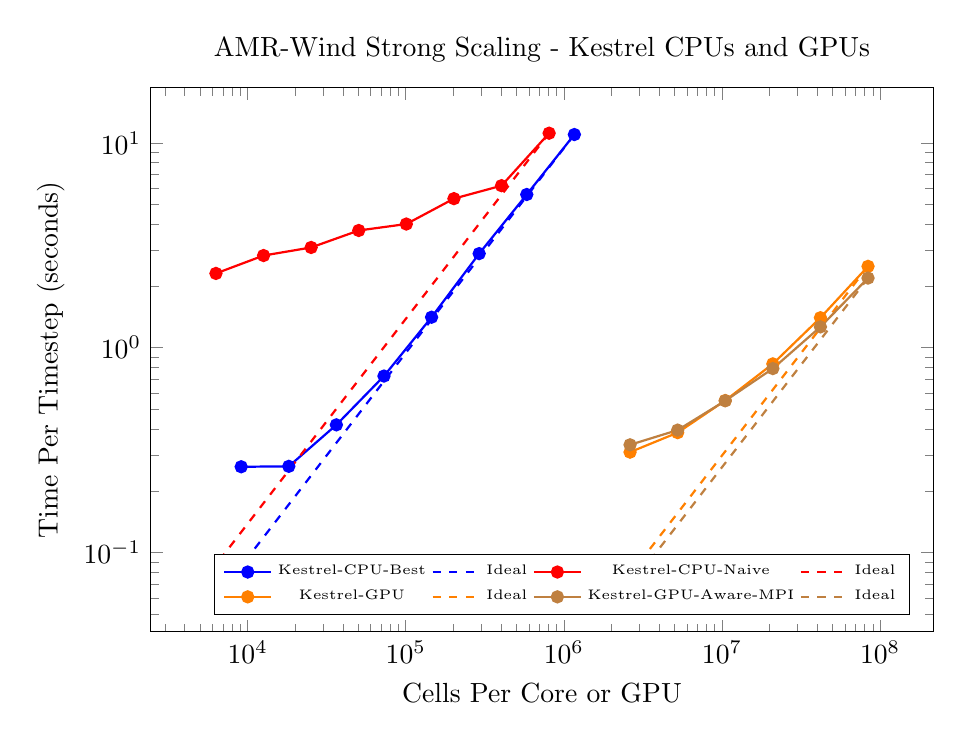
\begin{tikzpicture}
\begin{loglogaxis}[
  title=AMR-Wind Strong Scaling - Kestrel CPUs and GPUs,
  xlabel={Cells Per Core or GPU},
  ylabel={Time Per Timestep (seconds)},
  legend pos=south east,
  legend columns=4,
  legend style={font=\tiny},
  width=0.95\linewidth,
  height=0.7\linewidth,
  every axis plot/.append style={thick},
  /pgf/number format/.cd,
        use comma,
        1000 sep={},
]

%Kestrel-CPU
\addplot[blue, mark=*, mark options={solid}] coordinates {
  (1165084.4444444445, 10.984)
  (582542.2222222222, 5.5981000000000005)
  (291271.1111111111, 2.8806000000000003)
  (145635.55555555556, 1.4091)
  (72817.77777777778, 0.727205)
  (36408.88888888889, 0.42018500000000003)
  (18204.444444444445, 0.26353)
  (9102.22222222, 0.262245)
};

%Kestrel-CPU ideal
\addplot[blue, mark=none, dashed] coordinates {
  (1165084.4444444445, 10.984)
  (9102.22222222, 0.0858125)
};

%Kestrel-CPU-Naive
\addplot[red, mark=*, mark options={solid}] coordinates {
  (806596.9230769231, 11.151000000000002)
  (403298.46153846156, 6.1819500000000005)
  (201649.23076923078, 5.34305)
  (100824.61538461539, 4.0163)
  (50412.307692307695, 3.7354999999999996)
  (25206.153846153848, 3.08605)
  (12603.076923076924, 2.81844)
  (6301.53846154, 2.3049000000000004)
};

%Kestrel-CPU-Naive ideal
\addplot[red, mark=none, dashed] coordinates {
  (806596.9230769231, 11.151000000000002)
  (6301.53846154, 0.08711719)
};

%Kestrel-GPU
\addplot[orange, mark=*, mark options={solid}] coordinates {
  (83886080.0, 2.4955000000000003)
  (41943040.0, 1.4012499999999999)
  (20971520.0, 0.8340099999999999)
  (10485760.0, 0.55235)
  (5242880.0, 0.38498)
  (2621440.0, 0.30915)
};

%Kestrel-GPU ideal
\addplot[orange, mark=none, dashed] coordinates {
  (83886080.0, 2.4955000000000003)
  (2621440.0, 0.07798438)
};

%Kestrel-GPU-Aware-MPI
\addplot[brown, mark=*, mark options={solid}] coordinates {
  (83886080.0, 2.1881)
  (41943040.0, 1.2637500000000002)
  (20971520.0, 0.7911699999999999)
  (10485760.0, 0.55082)
  (5242880.0, 0.396165)
  (2621440.0, 0.33575499999999997)
};

%Kestrel-GPU-Aware MPI ideal
\addplot[brown, mark=none, dashed] coordinates {
  (83886080.0, 2.1881)
  (2621440.0, 0.06837812)
};

\legend{Kestrel-CPU-Best, Ideal, Kestrel-CPU-Naive, Ideal, Kestrel-GPU, Ideal, Kestrel-GPU-Aware-MPI, Ideal}
\end{loglogaxis}
\end{tikzpicture}
\caption{Strong scaling of \texttt{abl\_godunov} case on Kestrel CPUs and GPUs. The CPU case has 83,886,080 cells and the GPU case has 335,544,320 cells which is 4x larger than the CPU case. The naive CPU case has all 104 CPU cores per node on Kestrel in use on nodes with a single NIC. The regular CPU case is using 72 cores per node with 2 NICs per node with specific process bindings.}
\label{fig:kestrel-strong-scaling-abl-oct-2025}
\end{figure}

\end{document}